\documentclass[uplatex,dvipdfmx,a4paper,10pt]{jsarticle}

\usepackage{amsmath,amsthm,amssymb}
\usepackage[dvipdfmx]{graphicx}
\usepackage{bm}
\usepackage{ascmac}
%
\usepackage{multirow}
\usepackage{wrapfig}
%
\pagestyle{empty}
%% 高さの設定
\setlength{\textheight}{\paperheight}   % ひとまず紙面を本文領域に
\setlength{\topmargin}{-5.4truemm}      % 上の余白を20mm(=1inch-5.4mm)に
\addtolength{\topmargin}{-\headheight}  % 
\addtolength{\topmargin}{-\headsep}     % ヘッダの分だけ本文領域を移動させる
\addtolength{\textheight}{-40truemm}    % 下の余白も20mmに%% 幅の設定
\setlength{\textwidth}{\paperwidth}     % ひとまず紙面を本文領域に
\setlength{\oddsidemargin}{-5.4truemm}  % 左の余白を20mm(=1inch-5.4mm)に
\setlength{\evensidemargin}{-5.4truemm} % 
\addtolength{\textwidth}{-40truemm}     % 右の余白も20mmに

%
\abovecaptionskip=-1pt
%\belowcaptionskip=-1pt
%
\renewcommand{\baselinestretch}{0.9} % 全体の行間調整
\renewcommand{\figurename}{Fig.}
\renewcommand{\tablename}{Tab.}
\renewcommand{\thefootnote}{\fnsymbol{footnote}}
%
\makeatletter 
\def\section{\@startsection {section}{1}{\z@}{1.5 ex plus 2ex minus -.2ex}{0.5 ex plus .2ex}{\large\bf}}
\def\subsection{\@startsection{subsection}{2}{\z@}{0.2\Cvs \@plus.5\Cdp \@minus.2\Cdp}{0.1\Cvs \@plus.3\Cdp}{\reset@font\normalsize\bfseries}}
\makeatother 
%
% \graphicspath{{../../figures//}}
%
\begin{document}

%%%%%%
% はじめに
%%%%%%
\begin{center}
{\LARGE \textgt{MD シミュレーションによるネットワークポリマーのゴム弾性}}
\end{center}

\begin{flushright}
東亞合成 ${}^\circ$佐々木裕
\end{flushright}

\renewcommand{\thefootnote}{\fnsymbol{footnote}}
\footnote[0]{
{\bf Evaluation of Rubber Elasticity of Network Polymer by MD Simulation} \\
\underline{Hiroshi SASAKI} (Toagosei Co., Ltd. 8, Showa-Cho, Minato-ku, NAGOYA 455-0026, JAPAN)\\
Tel: +81-52-611-9923, e-mail: hiroshi\_sasaki$@$mail.toagosei.co.jp
}

\vspace{-1.2\baselineskip}
\section{はじめに}
% 軽量化を目指した新規複合材料の開発において高分子材料の高靭性化は重要な問題であり、力学特性に優れたネットワークポリマーの開発が進んでいる。そのなかでも、

破壊靭性が高いゴム系材料は、フィラー同士の相互作用のような比較的大きなスケールの構造から、フィラー界面近傍での拘束領域のような中間的なスケール、さらには、ネットワーク構造の均一性のようなミクロなスケールに至るマルチスケールの事象が階層的に組み合わさりマクロ特性に大きな影響を与えることが知られている。

ゴムの大きな破壊靭性値について、 ヒステリシスロスの存在が亀裂進展に伴うエネルギー開放量を減少させ、その結果、亀裂の進展が抑制されるというモデルがAndrewsに提案されている~\cite{Andrews1977}。
ゴムへのフィラーの添加~\cite{Igarashi2013}においては大きなヒステリシスが存在し、その高靭性メカニズムはこの考え方に合致している。
この効果はメゾスケール領域での挙動であると考えられているが、ヒステリシス挙動はこのスケールでしか発現しないのであろうか。
我々は、分子鎖描像のようなミクロな領域においても粘弾性緩和でのエネルギー散逸を設計することでエラストマー材料の破壊耐性を向上し、しなやかな強さを付与できる可能性が残されているのではないかと考えている。

ゴム弾性の古典的なモデルとして、結節点のミクロな変形がマクロな変形と相似でアフィン変形するとした「ネオ・フッキアンモデル」が知られている。
この発展形として、結節点の揺らぎに注目しミクロな変形がマクロと異なるとした「ファントムネットワークモデル」が提案されている。
我々は、この結節点のゆらぎ由来の散逸が、ミクロなスケールでの粘弾性的なエネルギー散逸モデルとなりうるのではないかと考えている。

本報告では、規則構造ネットワークのユニットセル間における規則性をランダムへと変えることで、「ファントムネットワークモデル」を再現できるシミュレーション系の構築を目指し、平衡構造での鎖の挙動、及び、大変形時の挙動に注目した検討結果について報告する。

\begin{wrapfigure}{r}[5mm]{60mm}
	\vspace{-2\baselineskip}
		\begin{center}
		\includegraphics[width=50mm]{./fig/Network.png}
		\caption{Topological NW Model}
		\label{fig:topo}
		\end{center}
	\vspace{-2\baselineskip}
\end{wrapfigure}

\section{シミュレーション}

\subsection{ネットワークモデルの作成}

任意の分岐数$f$($f=3\sim6$)の結節点からなる規則構造を有するネットワークより、以下のアルゴリズムでランダムな結合性を導入した。
\vspace{-2mm}
\begin{enumerate}
\item
任意の分岐数のトポロジーモデルを作成(Fig. \ref{fig:topo})。
\item
代数的連結性を指標として連結性を維持しながらストランド交換し、結節点の結合性にランダム性を導入(Fig. \ref{fig:exc})。
\item
トポロジーモデルに対応して実空間の構造からストランドを除去。
\end{enumerate}

\begin{wrapfigure}{r}[0mm]{80mm}
	\vspace{-1\baselineskip}
		\begin{center}
		\includegraphics[width=80mm]{./fig/ボンド交換.png}
		\caption{Strand Exchange Procedure}
		\label{fig:exc}
		\end{center}
	\vspace{-2\baselineskip}
\end{wrapfigure}

\subsection{MD シミュレーション}

上記にて生成したネットワークをOCTA 上の COGNAC シミュレーターにより MD シミュレーションを行った。


\section{結果と考察}

% \subsection{トポロジーモデルの結節点のランダム性の評価}

% % 上記のモデルにおいて、
% ストランド交換を繰り返し(100,000 回) 代数的連結性の分布関数を得、最頻値近傍のトポロジーモデルを実空間での初期構造とした。

\subsection{ストランドの末端間距離 $\langle \bm{R} \rangle$ の分布関数}

初期緩和後のストランドの末端間距離は初期設定と比較して伸びており、ファントムネットワークモデルで予想される振る舞いとほぼ合致した。

\subsection{ファントムネットワークの緩和}

ステップ変形により応力緩和を評価し、ネットワークの緩和について調べた。

\vspace{-2mm}

\bibliographystyle{../achemso}
\bibliography{D:/Dropbox/Bibliography/library.bib}

\end{document}